%%% In this section, you will describe all of the various artifacts that you will generate and maintain during the project life cycle. Describe the purpose of each item below, how the content will be generated, where it will be stored, how often it will be updated, etc. Replace the default text for each section with your own description. Reword this paragraph as appropriate.

\subsection{Major Documentation Deliverables}


\subsubsection{Project Charter}
This document will be updated at the end of each sprint, since that is when we will update our design, risks, costs, and other items included in the project charter. The initial version will be delivered on $11^{th}$ October 2021. The final version will be delivered at the end of November or early December. 

\subsubsection{System Requirements Specification}
This document will be updated if we make changes to the core functionality of the robot. This seems unlikely, since the robot will adhere to the rules of the robotics competition. The initial version will be delivered on $25^{th}$ October 2021. The final version will be delivered at the end of the semester 

\subsubsection{Architectural Design Specification}
This document will be updated if changes are made to the overall design of the robot. Initial version will be delivered on $15^{th}$ November 2021. The final version will be delivered at the end of the semester 

\subsubsection{Detailed Design Specification}
This document will be updated once we have specific details of the robot, and its mechanisms. Any minor changes made to the robot will be recorded. The initial and final version will be delivered at the end of the semester. 

\subsection{Recurring Sprint Items}


\subsubsection{Product Backlog}
Evan Cornish will be responsible for the task of maintaining the product backlog. Each sprint the tasks that are completed will be reported in the group meetings, and the tasks will be moved ot the completed section.
Our backlog will be maintained on the Jira software. Backlog items will be added and marked complete by a group vote. 

\subsubsection{Sprint Planning}
There will be a meeting every 2 weeks solely for sprint planning purposes. At this meeting tasks that need to be accomplished will be voted upon, and then responsibilities will be assigned based on a group decision as well.
There are 5 remaining sprints available during the Fall semester not counting winter break. Over winter break our goal is to do 1 more sprint, taking 1 week off for Christmas.
There are 5 sprints available before the competition date of April 2nd. That means our total remaining sprints is 11 or 12 depending on how many we manage over winter break.

\subsubsection{Sprint Goal}
There is no customer in our case. Our sprint goals will be decided on a combination of group voting with emphasis given to our 2 computer engineers, and consulting with Dr. McMurrough on our path.

\subsubsection{Sprint Backlog}
Zach Trumbaturi is in charge of making sure that our tasks are completed in the order that will give us the highest chance of scoring the most points possible. The administrative tasks of maintaining the backlog will be maintained by Evan Cornish, but all members are welcome to update the backlog. Evan Cornish's role is to certify that the backlog is correct and up to date at all times.

\subsubsection{Task Breakdown}
Tasks will be assigned by the group based on individual strengths. Time spent on tasks will either be documented manually with a spreadsheet, or using the myhours app from myhours.com or something similar to maintain a record.

\subsubsection{Sprint Burn Down Charts}
Evan Cornish will be responsible for generating the sprint burn down chart for each sprint. At the end of each sprint there will be a meeting where each member will report to him their hours spent on each task for him to maintain the records. 

%%%%%%%%%%%%%%%%%%%%%%%%%%%%%%%%%%%%%%%%%%%%%%%%%%%%%%%%%%
%  BE SURE TO UPDATE THE IMAGE CAPTION
\begin{figure}[h!]
    \centering
    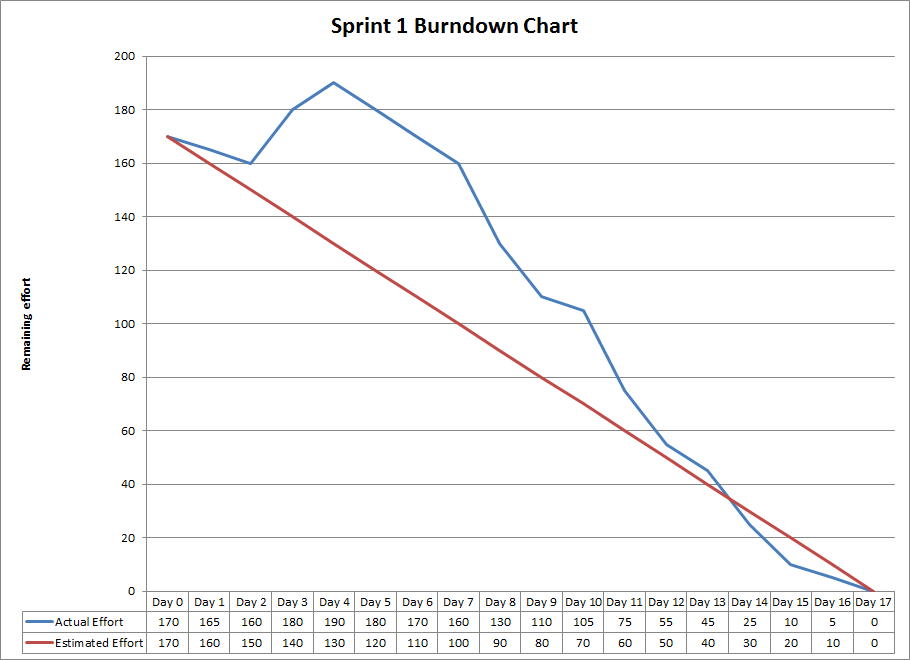
\includegraphics[width=0.5\textwidth]{images/burndown.png} % Image
    \caption{Example sprint burn down chart} % Caption
\end{figure}

\subsubsection{Sprint Retrospective}
At the end of each sprint there will be a meeting to discuss accomplishments, failures, and effort expended. 

\subsubsection{Individual Status Reports}
Statuses for each team member will be their completed tasks and how far into completion they are on unfinished tasks. These status reports will be given to the entire group, and notes and updates made to our Jira board accordingly by Evan Cornish.

\subsubsection{Engineering Notebooks}
engineering notebooks will be updated at a minimum on a weekly basis for each team member. There are 2 sub teams in the beginning for our sprint consisting of Evan and Zach on subteam A and Kartikey, Osama and Paola on subteam B. Each subteam has a task that can be accomplished in parallel. As such each member from either subteam can sign off as a witness for that same members engineering notebook.

\subsection{Closeout Materials}


\subsubsection{System Prototype}
The final system prototype will include a working tethered underwater robot capable of all kinds of movements ranging from forward, backward, sideways to sinking down to bottom and rising to the surface of a water body. The final prototype will also include a display of mechanism capable of collecting trash and dropping it at a desired place.  

The offsite demonstration will take place at the IEEE robotics competition in Houston.  

\subsubsection{Project Poster}
The project poster will include an animated picture of the robot highlighting the thrusters and trash collecting mechanism with animated picture of all team members standing around it in a testing field.  

The project poster will be delivered by UTA Innovation Day.

\subsubsection{Web Page}
The web page will include the project poster, introduction of the project along with IEEE robotics competition introduction, and a segment with team member's introductions. It will be made available to public along with updates on the making of this underwater robot. The webpage will me made available throughout the project and will be delivered by the end of $3^{rd}$ sprint cycle.  

\subsubsection{Demo Video}
The demo video will include the robot successfully moving through three rings of different diameters (first one being largest and last one being smallest) at bottom of a pool. Furthermore, the robot will be seen collecting trash box and bringing it to a platform on the surface of the said pool.  

The length of video will range anywhere from 15 to 30 minutes depending on the power provided to the robot.  

\subsubsection{Source Code}
The team has decided to use GitHub as version control system to maintain source code. The source code will be delivered to binaries only. After the competition is concluded the source code will be made available to the public under the MIT license. The terms will be listed at the top of each source code file.  

\subsubsection{Source Code Documentation}
The team will use Doxygen to generate source code documentation. The final documentation will be provided in browsable HTML format.  

\subsubsection{Hardware Schematics}
The hardware schematics is still a topic of discussion, and nothing is confirmed as of now. The team is considering using a Raspberry pi and Arduino Microcontroller to control the thrusters and camera and wire them up with the system control.  

This section will be updated in the next sprint cycle.  

\subsubsection{CAD files}
This project will involve mechanical design and a 3D printer will be used to print certain components for the mechanical frame of the robot.  

The team will use software named 'tinkercad' to generate files for 3D printing and the file format provided in the closeout material will be STL.  

\subsubsection{Installation Scripts}
Not applicable  

\subsubsection{User Manual}
Since this project is for a robotics competition and the team will do a live demonstration of the robot and its capabilities, a user manual won't be provided or necessary.  
